\documentclass[margin=10pt]{standalone}
\usepackage{circuitikz}
\begin{document}
    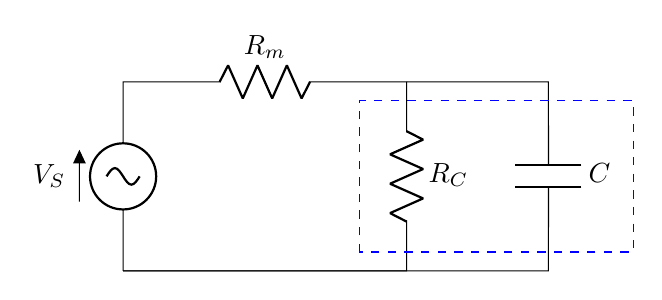
\begin{tikzpicture}[scale=1.2]
    %--------start graphics code --------
    %\draw[step=0.5,very thin,black!20] (-1,-0.5) grid (6,2.5);
    \path (0,0) coordinate (ref_gnd);
    \draw
        (ref_gnd) to[sinusoidal voltage source=$V_S$] ++(0,2)
            to[R=\(R_m\)] ++(3,0)
            to[R=\(R_C\)] ++(0,-2)
        -- (ref_gnd);
    \path (3,2) coordinate (cap);
    \draw
        (cap) to ++(1.5,0)
            to[C=\(C\)] ++(0,-2)
        -- (ref_gnd);
    \draw [dashed,blue] (1,0) ++(1.5,0.2) rectangle ++(2.9,1.6);
    %--------end graphics code ----------
    \end{tikzpicture}
\end{document}
